\section{Modelling Customer Behaviours}
\label{sec:model}

Customers' behaviour evolves over time as they respond to business offering and adjust to their own demand. We would like to represent the various behaviour dynamics of a collection of customers by panel data, and employ the Markov chain model to describe these data. In addition, we use the mixture model to find Markov states, each of which defines a partition of the behaviours observable within a single time interval.

\subsection{Representing Behaviours by Features}

A \textit{feature} is an individual measurable property of a behaviour being observed, and choosing informative features is crucial for effective clustering. For example, to measure how often the pupil uses Whizz online tutorial, we can define the time spent or number of visits within a month as the feature. For each customer, we define multiple features to capture his behaviours of various aspects within a time interval. Suppose we are interested in studying behaviours of $n$ customers in $T$ discrete consecutive time periods, and define $m$ features, then we denote the feature data as a sequence:
\begin{equation}
\label{eq:customerJourney}
\left\lbrace \mathbf{X}_1, ~\mathbf{X}_2, ~\dots, ~\mathbf{X}_t, ~\dots, ~\mathbf{X}_T \right\rbrace,
\end{equation}
in which the $t$-th element $\mathbf{X}_t = (x_{ij}^t) \in \mathbb{R}^{m \times n}$ is a matrix for all $t=1,2,\dots,T$. In addition, we denote the features of customer $j$ at the $t$-th time interval by the $j$-th column of $\mathbf{X}_t$ by $\mathbf{x}_{tj} = [x_{1j}^t ~x_{2j}^t ~\cdots ~x_{mj}^t]^\top$.

\subsection{Customer Journeys and Markov Chain}

Customer journeys reflect their feature dynamics over time, denoted as (\ref{eq:customerJourney}). One practical challenge of computing such sequence of matrices is to resolve the inconsistency present in journeys of different customers. The inconsistency refers to the problem that the time intervals for different customers being alive in the services are not aligned, so that their features are not comparable. Moreover, it is highly likely to have significant missing information within specific time intervals for customers who have not yet entered the service or have already churned. To resolve the inconsistency, we align and aggregate customers' features by \textit{customer month} rather than calendar month. Doing so enables the effective modelling using Markov chain.

\subsubsection{Customer Month}

Splitting pupils' behaviours into monthly time periods makes most sense provided the business settings at Whizz. Pupils subscribe to access Whizz products on a 1-month contract, and make the choice to leave the service at the end of each subscription. If no action is taken, a renewal will be made by default.

Due to the inconsistency present in journeys of different customers, we align their features by switching the reference from calendar month to customer month. This is illustrated by an example in \Cref{fig:customerMonth}. It provides much cleaner and more sensible data for modelling task. 

\begin{figure}[!h]
\centering
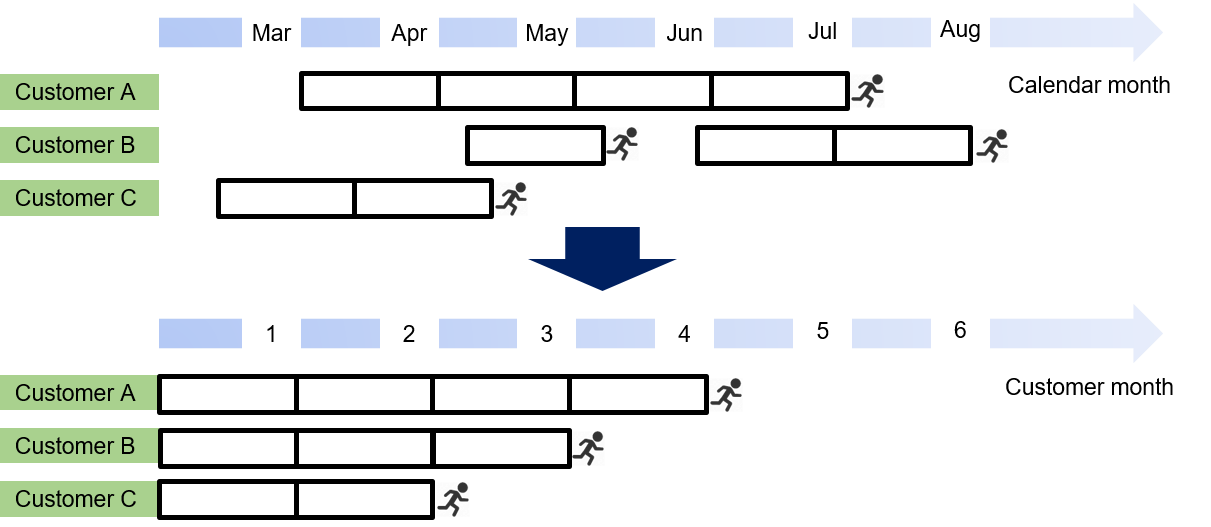
\includegraphics[scale=.75]{CustomerMonth.png}
\caption{Change reference from calendar month to customer month. Customer A, B and C have very different journeys in the sense of subscription start and end dates. Each block represents customer's monthly features. Under calendar month reference, we have to choose studying months from March to August to cover all activities. This choice results in irregular temporal distribution of missing information for all 3 customers. After changing the reference to customer month, features are aligned by customer month and therefore comparable. Moreover, the missing information only occurs after the customer churns. It can also handle discontinuous subscriptions like the case of customer B.}
\label{fig:customerMonth}
\end{figure}

\subsubsection{Markov Chain - Dynamic Model for Behavioural Changes}

We assume that customers with intentions to churn exhibit different behaviours than others do. Behaviours are different distributionally, and generated from a finite number of \textit{states}. Then the discrete time behaviour of each customer results in a chain of states over time. This formulates into a discrete-time Markov chain with states transiting over time, where each state emits distinguishable behaviour distribution from others. An example is given in \Cref{fig:markovChain}. In brief, a Markov chain is a stochastic process characterised by \textit{transition} and \textit{emission} probabilities.

\begin{figure}[!h]
\centering
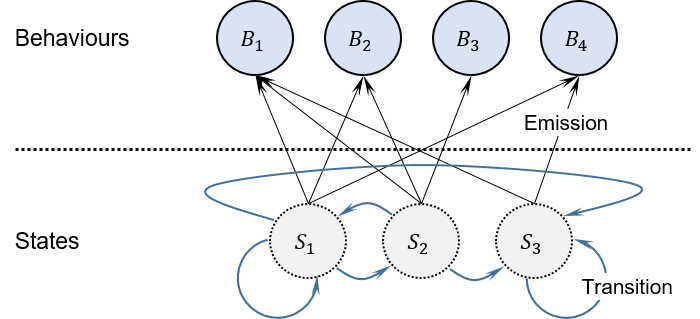
\includegraphics[scale=.75]{Markov.png}
\caption{Behaviours emitted from Markov states. States $S_1$, $S_2$ and $S_3$ generate differently distributed behaviours. For example, $S_1$ generates $\{ B_1, ~B_2, ~B_4\}$ while $S_3$ produces $\{ B_1, ~B_4\}$. Even if the two states can generate the same set of behaviours, the emission probabilities can be different, thus still resulting in different behaviour distributions. States transit between each other over time stochastically.}
\label{fig:markovChain}
\end{figure}

\paragraph*{Transition}

Consider the behavioural journey of customer $j$, which is represented by a sequence of feature data $\{ \mathbf{x}_{tj} \}_{t=1}^{T}$. At time interval $t$, feature $\mathbf{x}_{tj}$ is an instance from a distribution generated by a state. Let's denote the time sequence of generative states as $\{ s_{t}(j) \}_{t=1}^{T}$. In a Markov chain setting the sequences are defined stochastically, with the next state being conditionally dependent on the present state, but not any further previous history. This is known as \textit{Markov property}. 

If we define a finite set of states by $\mathcal{S} = \{ S_q \}_{q=1}^Q$, then $s_t (\cdot)$ is a map from $\mathbb{N}$ to $\mathcal{S}$. Due to the Markov property, successive states are linked together with the (conditional) \textit{transition probability matrix} defined as:
\begin{subequations}
\begin{equation}
A_t = (a_{pq}^t) \in [0,1]^{Q \times Q}, 
\end{equation}
with
\begin{equation}
a_{pq}^t = \mathbb{P} \left( s_{t+1} = S_p | s_t = S_q \right).
\end{equation}
\label{eq:transition}
\end{subequations}
If we assume time-homogeneity or \textit{stantionarity} of the Markov chain, then we can remove the time subscript from the notations because the parameters describing all probabilistic transitions are themselves constant.

\paragraph*{Emission}
\label{sec:emission}

Recall that feature data $\{ \mathbf{x}_{tj} \}_{t=1}^{T}$ observed are instances from some distribution. We introduce a generic notation for observed sequence of features, $\{ \mathbf{o}_{t} \}_{t=1}^{T}$, where $\mathbf{o}_t = [o_{t1} ~o_{t2} ~\cdots ~o_{tm}]^\top$. The sequence of observations are generated in the following way:
\begin{enumerate}
\item At each time step, the system generates a state $s_t$ according to the state-to-state transition probability matrix $A_t$.
\item Once the state $s_t$ has been generated, the system generates a cluster $c_t$ according to a state-to-cluster emission probability distribution $\pi(s_t,c_t)$. Suppose we define a finite collection of clusters $\mathcal{C} = \{ C_k \}_{k=1}^K$, then we denote:
\begin{equation}
\pi_{qk} = \pi(S_q, C_k) = \mathbb{P} \left( c_t = C_k | s_t = S_q \right).
\end{equation}
\item Once the cluster $c_t$ have been determined, an observation vector $\mathbf{o}_t$ is produced probabilistically according to some cluster-specific distribution $\phi(\mathbf{o}_t | \theta (s_t, c_t))$, where $\theta (s_t, c_t)$ denotes the distribution parameters. We write,
\begin{equation}
\phi(\mathbf{o}_t | \theta_{qk}) =  \phi(\mathbf{o}_t | \theta (S_q, C_k)) = \mathbb{P} \left( \mathbf{o}_t | s_t = S_q, c_t = C_k \right).
\end{equation}
\label{eq:phi}
\end{enumerate}
Given the generative process described above, we can now model the state-to-observation emission probability by a mixture of densities:
\begin{subequations}
\begin{align}
b_q (\mathbf{o}_t) & = \mathbb{P} \left( \mathbf{o}_t | s_t = S_q \right) \\
 & = \sum_{k=1}^K  \mathbb{P} \left( c_t = C_k | s_t = S_q \right) \mathbb{P} \left( \mathbf{o}_t | s_t = S_q, c_t = C_k \right) \\
 & = \sum_{k=1}^K \pi_{qk} \phi(\mathbf{o}_t | \theta_{qk}).
\end{align}
\label{eq:emission}
\end{subequations}

\subsubsection{Decoding the Markov Chain}

The problem is how to estimate the transition probabilities and parameters in the emission term, $A_t$ and $(\pi, \theta)$ from the observations $\mathbf{X}_t$. Our strategy is to split this decoding process into two separate steps, where we first make inference on emission and then uncover the temporal structure configured by transition.

\paragraph*{Decoding Emission}

Ideally from the perspective of practical application of the model, we wish to encode a finite number of states representing different levels of churn risk. As a consequence, the prediction task is to find out the state that the pupil belongs to and therefore assigning the associated risk label. Hence, we choose not to infer states purely from observed behavioural data, but define states by also incorporating churn outcome information. At high level, we take two steps to estimate the parameters in the emission term:
\begin{enumerate}
\item We look at the behavioural distribution without conditioning on state, namely,
\begin{equation}
b(\mathbf{o}_t) = \mathbb{P} (\mathbf{o}_t) = \sum_{k=1}^K \mathbb{P} (c_t = C_k) \mathbb{P} (\mathbf{o}_t | c_t = C_k) = \sum_{k=1}^K \pi_k \phi(\mathbf{o}_t | \theta_k).
\label{eq:bo}
\end{equation}
Then we estimate $\{ \pi_k, \theta_k \}_{k=1}^K$ from observed feature data $\mathbf{X}_t$ with pre-defined multivariate kernel density $\phi(\cdot)$. This will be elaborated in section \ref{sec:mixtureModel}.

\item The previous step gives not only the weights $\pi$ and cluster density $\phi(\cdot | \theta)$, but also a consequential cluster assignment of all customers. If we know the churn outcome for all customers, then we can calculate the proportion of churned customers, or churn rate, within each cluster. Thereafter, we can form states by grouping together clusters of similar level of churn rate.

Formally, we define the set of customers who have been assigned into cluster $C_k$ as
\begin{equation}
\mathcal{N}_k^t = \left\lbrace j :~ j \text{ is assigned into } C_k \text{ at time } t \right\rbrace.
\end{equation}
Meanwhile, we define the churn outcome information by a set
\begin{equation}
\mathcal{N}_\text{churn}^t = \{j: ~j \text{ churns at } t+1 \},
\end{equation}
so that the cluster churn rate is defined as
\begin{equation}
\lambda_k^t = \frac{\vert \mathcal{N}_k^t \cap \mathcal{N}_\text{cancel}^t \vert}{\vert  \mathcal{N}_k^t \vert}.
\label{eq:clusterChurn}
\end{equation}
Once the churn rates of all $K$ clusters, $\{ \lambda_k^t \}_{k=1}^K$, are computed, we group them and form $Q$ states. Typically $Q$ is much smaller than $K$. We denote the set of clusters consisting state $S_q$ as,
\begin{equation}
\mathcal{K}_q^t = \left\lbrace k :~ C_k \text{ is emitted from } S_q \text{ at time } t \right\rbrace.
\end{equation}
\end{enumerate}
Afterwards, we can revisit the calculation for the state-to-observation emission probability $b_q(\mathbf{o}_t)$. Note that by the way we define state, we have
\begin{equation}
\pi_{qk} = \mathbb{P} \left( c_t = C_k | s_t = S_q \right) = \frac{\vert \mathcal{N}_k^t \vert}{\sum_{l \in \mathcal{K}_q^t} \vert \mathcal{N}_l^t \vert} \mathbbm{1}_{\{ k \in \mathcal{K}_q^t \}},
\end{equation}
where $\mathbbm{1}_{\{\cdot\}}$ is the indicator function. Then
\begin{equation}
b_q (\mathbf{o}_t) = \sum_{k=1}^K \pi_{qk} \phi(\mathbf{o}_t ; \theta_{qk}) = \sum_{ k \in \mathcal{K}_q^t } \frac{\vert \mathcal{N}_k^t \vert}{\sum_{l \in \mathcal{K}_q^t} \vert \mathcal{N}_l^t \vert} \phi(\mathbf{o}_t | \theta_{k}).
\end{equation}

\paragraph*{Decoding Transition}

We define the set of customers who transit from $S_p$ at $t$ to $S_q$ at $t+1$ as
\begin{equation}
\mathcal{Q}_{q \rightarrow p}^t = \left\lbrace j: ~s_t(j) = S_q, ~s_{t+1}(j) = S_p \right\rbrace.
\end{equation}
We assume that customers' behaviours are i.i.d. samples from the generating process, then the maximum likelihood estimate of the transition probability is
\begin{equation}
\hat{a}^t_{pq} = \frac{\vert \mathcal{Q}_{q \rightarrow p}^t \vert}{\sum_{l=1}^Q \vert \mathcal{Q}_{q \rightarrow l}^t \vert}.
\end{equation}
If the Markov chain is assumed to be stationary, then we estimate
\begin{equation}
\hat{a}_{pq} = \frac{\sum_{t=1}^{T-1} \vert \mathcal{Q}_{q \rightarrow p}^t \vert}{\sum_{t=1}^{T-1} \sum_{l=1}^Q \vert \mathcal{Q}_{q \rightarrow l}^t \vert}.
\label{eq:transition}
\end{equation}

\subsection{Probabilistic Clustering Using Mixture Model}
\label{sec:mixtureModel}

A critical step of the state-cluster-observation Markov chain is the mixture model that describes the probabilistic assignment of observations to clusters. Practical calibration of the mixture model faces many choices such as the kernel density $\phi(\cdot)$, the number of clusters $K$, etc. A fundamental model setting is however the choice of frequentist or Bayes approach to estimate model parameters. We choose specifically the \textit{Dirichlet Process Mixture} setting which has two important features:
\begin{enumerate}
\item It is Baysian and treats $\theta$ as a random variable, of which distributions will be updated from a prior as observed data coming in. 
\item The Dirichlet process (DP) is used as a nonparametric prior resulting in that the number of clusters is random and grows as new data are observed.
\end{enumerate}
The benefits of this model choice are massive. It does not view the observed data as infinitely available as independent replicates like frequentists, so that it does not worry about the unobserved data and can be updated with new data coming in. Moreover, it infers the number of clusters from observed data, and opens the opportunities of finding new clusters as more data are observed.

\subsubsection{Dirichelet Process Mixture Model}

\paragraph*{Definitions}

A Dirichelet Process (DP) is a distribution of a random measure. Let $G_0$ be a base distribution (measure) for our cluster density parameter $\theta \in \Theta$, a measurable space, and let $\alpha$ be a positive, real-valued scalar. A random measure $G$ is then distributed according to \textit{Dirichelet Process} with scaling parameter $\alpha$ and base measure $G_0$:
\begin{subequations}
\begin{equation}
G \sim \text{DP}(\cdot | G_0, \alpha),
\end{equation}
if for all $K \in \mathbb{N}$, and all $\{ \Theta_1, \dots, \Theta_K \}$ finite partitions of $\Theta$:
\begin{equation}
\left( G(\theta_1), \dots, G(\theta_K) \right) \sim \text{Dir} \left( \alpha G_0(\theta_1), \dots, \alpha G_0(\theta_K) \right),
\end{equation}
where $\text{Dir}(\cdot)$ denotes the \textit{Dirichelet distribution}. The Dirichelet distribution is a distribution of the standard $K-1$ simplex. Let $\bm\pi = \{ \pi_k \}_{k=1}^K$ with $\sum_{k=1}^K \pi_k = 1$ and $\forall k: \pi_k \geq 0$, and let $\bm \alpha = (\alpha_1, \dots, \alpha_K)$ with $\alpha_1, \dots, \alpha_K \geq 0$. Then
\begin{equation}
\mathbb{P}(\bm\pi | \bm\alpha) = \text{Dir} (\alpha_1, \dots, \alpha_K) = \frac{1}{\text{Beta} (\bm\alpha)} \prod_{k=1}^K \pi_k^{\alpha_k-1} = \frac{\Gamma \left( \sum_k \alpha_k \right)}{\prod_k \Gamma(\alpha_k)} \prod_{k=1}^K \pi_k^{\alpha_k-1},
\end{equation}
where $\text{Beta}(\cdot)$ is the beta function, $\Gamma(\cdot)$ is the gamma function.
\label{eq:definitionDP}
\end{subequations}

\paragraph*{Clustering Effect}

We use DP as a prior to distribution of cluster parameter $\theta$:
\begin{equation}
\theta | G \sim G(\cdot) \quad\text{ and }\quad G \sim \text{DP} (\cdot | G_0, \alpha).
\label{eq:thetaDP}
\end{equation}
This model exhibits a ``clustering effect'' which enables us to infer number of clusters from data rather than pre-defining it. Suppose we independently draw $n$ random values $\theta^{(j)}$ from $G$ under the model (\ref{eq:thetaDP}), then Blackwell and MacQueen's urn representation theorem \cite{blackwellm73} states that, marginalising out the random measure $G$, the joint distribution of the collection of variables $\{\theta^{(1)}, \dots, \theta^{(n)}\}$ exhibits a clustering effect:
\begin{equation}
\mathbb{P} \left( \theta^{(j)} | \theta^{(1)}, \dots, \theta^{(j-1)} \right) \propto \alpha G_0 (\theta^{(j)}) + \sum_{l=1}^{j-1} \delta_{\theta^{(l)}} (\theta^{(j)}),
\end{equation}
where $\delta_{\theta^{(l)}} (\cdot)$ is a Dirac delta at ${\theta^{(l)}}$. Thus the variables $\{\theta^{(1)}, \dots, \theta^{(n)}\}$ are randomly partitioned according to which variables are equal to the same value. Moreover, let $\{ \theta_1, \dots, \theta_K \}$ denote the distinct values of the drawn samples $\{\theta^{(1)}, \dots, \theta^{(j-1)}\}$, let $\{\kappa_1, \dots, \kappa_{j-1}\}$ be the assignment variables such that $\theta^{(l)} = \theta_{\kappa_l}$. Then,
\begin{equation}
\mathbb{P} \left( \theta^{(j)} | \theta^{(1)}, \dots, \theta^{(j-1)} \right) \propto \frac{\alpha}{j-1+\alpha} G_0 (\theta^{(j)}) + \sum_{k=1}^{K} \frac{\vert \{ l: \kappa_l = k \} \vert}{j-1+\alpha}  \delta_{\theta^{(l)}} (\theta^{(j)}).
\end{equation}
This implies that the $j$-th draw has a probability of $(j-1)/(j-1+\alpha)$ to be exactly the same as some previously drawn value. This forms a natural clustering effect. In addition, with a probability of $\alpha/(j-1+\alpha)$ a new cluster will be produced with the new distinct value $\theta_{K+1}$. Hence the number of clusters is allowed to grow as new data are observed.

\paragraph*{Dirichelet Process Mixture Model}

Given the clustering effect exhibited in DP, we define the \textit{Dirichelet process mixture model} as:
\begin{equation}
\mathbf{o} | \theta \sim \phi(\cdot | \theta) \quad\text{ and }\quad  \theta | G \sim G(\cdot) \quad\text{ and }\quad G \sim \text{DP} (\cdot | G_0, \alpha),
\label{eq:DPMM}
\end{equation}
recall that $\mathbf{o}$ is the observed feature vector, we remove the time subscript $t$ since the mixture model holds for all time steps.

\subsubsection{Generative Process with Stick-Breaking Representation}

The definition of DP stated in (\ref{eq:definitionDP}) does not provide useful information of generating a DP in practice. Sethuraman \cite{sethuraman94} proposes the \textit{stick-breaking representation} to explicitly construct a DP. Suppose there are two infinite sets of independent random variables, $\beta_k \sim \text{Beta}(1, \alpha)$ and $\theta_k \sim G_0$, $\forall k \in \{1,2,\dots\}$. The stick-breaking representation of $G$ is:
\begin{subequations}
\begin{equation}
G(\cdot) = \sum_{k=1}^\infty \pi_k (\bm \beta) \delta_{\theta_k}(\cdot),
\end{equation}
where
\begin{equation}
\pi_k (\bm \beta) = \beta_k \prod_{l=1}^{k-1} (1-\beta_l).
\end{equation}
\end{subequations}
Note that by construction $\sum_{k=1}^\infty \pi_k (\bm \beta) = 1$. In the DP mixture model, $\bm\pi (\bm\beta) = \{ \pi_k (\bm \beta) \}_{k=1}^\infty$ gives the mixing proportions of mixture components represented by atoms $\{ \theta_k \}_{k=1}^\infty$. By far, we can describe the feature data generative process as follows:
\begin{enumerate}
\item Draw an infinite collection of $\beta_k | \alpha \sim \text{Beta} (1, \alpha)$, $\forall k \in \{1,2,\dots\}$.
\item Draw an infinite collection of $\theta_k | G_0 \sim G_0$, $\forall k \in \{1,2,\dots\}$.
\item For $j$-th data point, $j = 1,\dots, n$:
	\begin{enumerate}
	\item Draw $z^{(j)} | \bm\beta \sim \text{Mult} (\bm\pi (\bm\beta))$;
	\item Draw $\mathbf{o}^{(j)} | z^{(j)} \sim \phi ( \mathbf{o} | \theta_{z^{{(j)}}})$.
	\end{enumerate}
\end{enumerate} 

\subsubsection{Inference}

We use the variational inference for the Dirichelet process mixture model presented by Blei and Jordan \cite{blei2006}. In practice Dirichlet Process inference algorithm is approximated and uses a truncated distribution with a fixed maximum number of components, say $K_{\max}$, of $\beta$ and $\theta$. Nevertheless, the number of components actually used $K$ almost always depends on the data, and that $K \leq K_{\max}$.

\subsubsection{Predictive Density}

Based on model setting (\ref{eq:DPMM}), model configuration $(\phi(\cdot), \alpha, G_0)$ and observed feature data points $\{ \mathbf{x}_1, \dots, \mathbf{x}_n \}$, we are able to make inference on the posterior distribution $\mathbb{P}(\theta | \mathbf{x}_1, \dots, \mathbf{x}_n, \alpha, G_0)$. Afterwards, we can compute the predictive density:
\begin{equation}
\mathbb{P} (\mathbf{x} | \mathbf{x}_1, \dots, \mathbf{x}_n, \alpha, G_0) = \int \phi(\mathbf{x} | \theta ) \mathbb{P}(\theta | \mathbf{x}_1, \dots, \mathbf{x}_n, \alpha, G_0) \text{d} \theta.
\end{equation}

\subsection{Modelling Pipeline}
\label{sec:modelPipeline}

We summrise the processes of our modelling framework as a pipeline displayed in \Cref{tab:pipeline}. We will apply this pipeline to build a churn prediction model for Whizz.

\begin{table}[!h]
\centering
\footnotesize
\begin{tabular}{c|p{6cm}|p{3.5cm}|p{3.5cm}}
\hline
\textbf{No.} & \textbf{Process} & \textbf{Input} & \textbf{Output} \\
\hline
1 &
\textbf{Feature extraction}: extract informative feature data from historical records of pupils' activity, and represent them in the suitable data structure that can be fed into the behavioral model.&
Raw data from Whizz database that records pupils' ID, subscription history, activity history, etc. & 
Feature data represented by $\{\mathbf{X}_t\}_{t=1}^T$, as defined in (\ref{eq:customerJourney}). \\
\hline
2 &
\textbf{Feature distributional modelling}: choose the most suitable distributions for the all $m$ features to fit. Independent features can be modelled separately, while correlated features shall be modelled as a part of a multivariate distribution. &
Feature data represented by $\{\mathbf{X}_t\}_{t=1}^T$. & 
Density form $\phi(\cdot)$, as defined in (\ref{eq:phi}). (Note in this step we only propose the density form but not fit the distribution parameters.)\\
\hline
3 &
\textbf{Fitting DP mixture model}: by assuming behaviours are generated from a Dirichelet process mixtures, make inference on parameters based on observed features.&
Feature data represented by $\{\mathbf{X}_t\}_{t=1}^T$, feature density form $\phi(\cdot)$, and DP mixture model defined in (\ref{eq:DPMM}).& 
Posterior distribution $\mathbb{P}(\theta | \mathbf{X}, \alpha, G_0)$, a collection of clusters parametrised by different $\theta$. \\
\hline
4 &
\textbf{Fitting Markov chain}: use the identified clusters as well as churn outcome information to define states; uncover their transition probabilities. &
Identified probabilistic clusters with density $\{ \phi(\cdot | \theta_k) \}_{k=1}^K$; churn outcome. & 
A finite set of states $\mathcal{S} = \{S_q\}_{q=1}^Q$ and transition probability matrix $\{A_t\}_{t=1}^T$ \\
\hline
5.1 &
\textbf{Analytics on behaviours}: study the properties of pupils' behaviours such as the temporal transition probabilities, how each feature impact the level of churn risk, etc. &
States $\{S_q\}_{q=1}^Q$, transition $\{A_t\}_{t=1}^T$, cluster churn rate $\{ \lambda_k^t \}_{t,k}$ defined in (\ref{eq:clusterChurn}), etc. & 
Temporal state transition analysis, feature analysis, etc. \\
\hline
5.2 &
\textbf{Prediction on new pupils}: predict the level of churn risk for new pupils based on their behaviours with the observation-cluster-state probabilistic assignment trained from previous steps. &
States $\{S_q\}_{q=1}^Q$, clusters parametrised by $\mathbb{P}(\theta | \mathbf{X}, \alpha, G_0)$ for $\theta \in \{\theta_k\}_{k=1}^K$, cluster-state assignment. & 
State assignment for new pupils as well as their associated level of churn risk. \\
\hline
\end{tabular}
\caption{Modelling pipeline showing processes in sequence, along with the input and output of each modular process. The last two process 5.1 and 5.2 are independent from each other and are performed for different purposes.}
\label{tab:pipeline}
\end{table}